% arara: pdflatex: { interaction: nonstopmode }
% arara: biber
% arara: pdflatex: { interaction: nonstopmode }
% % arara: pdflatex: { interaction: nonstopmode }
% arara: clean: { extensions: [ log, aux, synctex ] }

\documentclass[aspectratio=169]{beamer}

\usepackage[utf8]{inputenc}
\usepackage{mathrsfs}
\usepackage[style=verbose,backend=biber]{biblatex}
\usepackage{tabularx}
\addbibresource{../master_thesis.bib}

\AtEveryCitekey{
	\clearfield{urlday}
	\clearfield{urlyear}
	\clearfield{urlmonth}
	\clearfield{urldate}
	\clearfield{timestamp}
	\clearfield{year}
	\clearlist{institution}
	\clearfield{type}
}
		

\usetheme{Boadilla}

\setbeamertemplate{navigation symbols}{}

\title[Master's Thesis Presentation]{Adopting Random Slicing for Riak Core}
\subtitle{Master's Thesis Presentation}
\author{Pascal Grosch}
\institute{TU Kaiserslautern}
\date{February 17, 2021}

\graphicspath{{../images/}}

\begin{document}
\frame{\titlepage}
\section{Introduction}
\begin{frame}
\frametitle{Introduction}
\begin{itemize}
\item cloud computing more and more prevalent
\item scalability is a big quality factor
\item distributing tasks to nodes influences scalability
\item Riak Core provides solutions to distribute tasks to nodes
\end{itemize}
\end{frame}

\begin{frame}
\frametitle{Riak Core (Lite)}
\begin{itemize}
\item open source implementation of the Dynamo architecture
\item framework for distributed systems
\item generates preference lists for keys
\item no actual replication mechanism
\item uses variant of Consistent Hashing
\item informs nodes of owner changes of keys
\item Riak Core Lite as a streamlined version
\end{itemize}
\end{frame}

\begin{frame}
\frametitle{Goals}
\begin{itemize}
\item analyze the influence of Consistent Hashing on the system structure
\item replace Consistent Hashing with Random Slicing
\item evaluate the performance differences
\end{itemize}
\end{frame}

\section{Consistent Hashing}
\begin{frame}
\frametitle{Consistent Hashing}
\begin{itemize}
\item uses hashing to map keys to nodes
\item hash space seen as ring
\item nodes are hashed to ring
\item keys are hashed to ring and mapped to the closest node
\item many different implementations used in practice
\end{itemize}
\end{frame}

\section{Riak Core's Consistent Hashing}
\begin{frame}
\frametitle{Riak Core's Consistent Hashing}
\begin{figure}
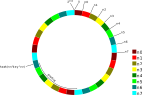
\includegraphics[height=0.8\textheight]{../images/consistent_hashing_example}
\end{figure}
\end{frame}

\begin{frame}
\frametitle{Changing the Cluster}
\begin{itemize}
\item on adding or removing nodes partitions are reassigned
\item claim algorithm responsible for load balancing and complete preference lists
\item administrator can change the number of partitions on the ring
\end{itemize}
\end{frame}

\begin{frame}
\frametitle{Constraints}
As pointed out by Scott Lystig Fritchie\footnote{https://www.infoq.com/articles/dynamo-riak-random-slicing/}
\begin{itemize}
\item partition number is fixed at initialization
\item number of Partitions has to be power of 2
\item partition size is fixed
\item claim assignment algorithm can lead to unbalanced workload
\item no weighting of nodes with different capacities
\end{itemize}
\end{frame}

\section{Random Slicing}
\begin{frame}
\frametitle{Random Slicing}
\begin{itemize}
\item alternative randomized data-distribution strategy
\item partitions $[0,1)$ range to sections
\item nodes own parts of the ring according to their relative capacity
\item hash function to real number in $[0,1)$
\item multiple sections can be handled by the same node
\item there is no fixed replication placement strategy
\end{itemize}
\end{frame}

\begin{frame}
\frametitle{Changing the Cluster}
\begin{figure}
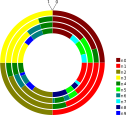
\includegraphics[height=0.8\textheight]{random_slicing_example}
\end{figure}
\end{frame}

\begin{frame}
\frametitle{Simple Replication Placement Strategies}
\begin{itemize}
\item Random Replication
	\begin{itemize}
	\item choose nodes randomly with their relative capacity as the probability
	\end{itemize}
\item Ring Rotation
	\begin{itemize}
	\item rotate the ring counter-clockwise under the key-index by size of sections
	\end{itemize}
\item Ring Jumping
	\begin{itemize}
	\item rotate the ring counter-clockwise under the key-index by size of the section the key points to
	\end{itemize}
\item all strategies require recomputation of replication placement after cluster changes
\end{itemize}
\end{frame}


\section{Adopting Random Slicing for Riak Core Lite}
\begin{frame}
\frametitle{Adopting Random Slicing for Riak Core Lite}
\begin{itemize}
\item system analysis shows the architecture relies on guarantees of Consistent Hashing
\item recreating system architecture not in scope
\item replacing Consistent Hashing as a prototype
\item only basic functionality kept
\item many optimizations lost
\item robustness lost
\end{itemize}
\end{frame}

\section{Evaluation}
\subsection{Evaluation Setup}
\begin{frame}
\frametitle{Evaluation Setup}
\begin{itemize}
\item rclref as in-memory key-value-store
\item rcl\_bench benchmarks operation throughput and latency
\item comparing replication placement strategies and partitioning algorithms
\item different cluster setups
\item different workloads
\end{itemize}
\begin{table}
\begin{tabularx}{\textwidth}{|l|X|}
\hline
Parameter & Values\\\hline
Riak Core Lite Configuration & ConsistentHashing, RandomSlicing\_Jumping, RandomSlicing\_Random, RandomSlicing\_Rotation\\
Cluster Configuration & 3 nodes, 4 nodes, 7 nodes, dynamic\\
Workload & read\_heavy, write\_heavy\\\hline
\end{tabularx}
\end{table}
\end{frame}

\subsection{Hypotheses}
\begin{frame}
\frametitle{Hypotheses}
\begin{itemize}
\item[H1] Random Replication is the best replication placement strategy regarding load balancing.
\item[H2] Random Replication is the best replication placement strategy regarding throughput.
\item[H3] The divergence from optimal load balancing is only marginally higher with Random Slicing than with Consistent Hashing.
\item[H4] The throughput in a static cluster is only marginally smaller with Random Slicing than with Consistent Hashing.
\item[H5] With Random Slicing handoff operations are faster than with Consistent Hashing.
\end{itemize}
\end{frame}

\subsection{Evaluation Results}
\begin{frame}
\frametitle{Results - Hypothesis 1}
\begin{table}
\begin{tabularx}{\textwidth}{|l|X|X|X|X|}
\hline
Configuration & Load Divergence Keys & Load Diversion Puts & Load Diversion Gets\\\hline
Overall\_RandomSlicing\_Jumping & 3.03\% & 3.66\% & 3.66\%\\
Overall\_RandomSlicing\_Random & 2.29\% & 2.70\% & 2.71\%\\
Overall\_RandomSlicing\_Rotation & 4.09\% & 3.58\% & 3.54\%\\
\hline
\end{tabularx}
\end{table}
\begin{itemize}
\item Random Replication has lowest load divergence in all configurations
\item data supports H1
\end{itemize}
\end{frame}

\begin{frame}
\frametitle{Results - Hypothesis 2}
\begin{itemize}
\item Ring Rotation clearly has the worst throughput
\item Random Replication and Ring Jumping show similiar throughput behavior in all configurations
\item data neither supports nor contradicts H2
\item may be a matter of scalability
\end{itemize}
\begin{figure}
\includegraphics[width=0.3\textwidth]{RandomSlicing_Random_C0_read_heavy_throughput}
\includegraphics[width=0.3\textwidth]{RandomSlicing_Jumping_C0_read_heavy_throughput}
\end{figure}
\end{frame}

\begin{frame}
\frametitle{Results - Hypothesis 3}
\begin{table}
\begin{tabularx}{\textwidth}{|l|X|X|X|X|}
\hline
Configuration & Load Divergence Keys & Load Diversion Puts & Load Diversion Gets\\\hline
Overall\_RandomSlicing\_Random & 2.29\% & 2.70\% & 2.71\%\\
Overall\_ConsistentHashing & 0.38\% & 3.24\% & 3.24\%\\
ConsistentHashing\_C2\_read\_heavy & 0.39\% & 0.39\% & 0.39\%\\
RandomSlicing\_Random\_C2\_read\_heavy & 0.16\% & 0.05\% & 0.07\%\\
ConsistentHashing\_C2\_write\_heavy & 0.38\% & 0.38\% & 0.40\%\\
RandomSlicing\_Random\_C2\_write\_heavy & 0.05\% & 0.05\% & 0.04\%\\
\hline
\end{tabularx}
\end{table}
\begin{itemize}
\item Overall load divergence extremely worse with Random Slicing
\item data strongly contradicts H3
\item for 7 nodes the load divergence with Random Slicing is less than the one with Consistent Hashing
\item may be a matter of scalability
\end{itemize}
\end{frame}

\begin{frame}
\frametitle{Results - Hypothesis 4}
\begin{itemize}
\item no significant differences in throughput in any configuration
\item H4 can be seen as plausible
\end{itemize}
\begin{figure}
\includegraphics[width=0.3\textwidth]{RandomSlicing_Random_C0_read_heavy_throughput}
\includegraphics[width=0.3\textwidth]{ConsistentHashing_C0_read_heavy_throughput}
\end{figure}
\end{frame}

\begin{frame}
\frametitle{Results - Hypothesis 5}
\begin{itemize}
\item shorter disruptions with Random Slicing than with Consistent Hashing for read-heavy workload
\item larger and more disruptions with Random Slicing than with Consistent Hashing for write-heavy workload
\item inconclusive results
\item additional and more refined benchmarks necessary
\item may be caused by cut out optimizations and edge cases
\end{itemize}
\begin{figure}
\includegraphics[width=0.3\textwidth]{RandomSlicing_Random_dynamic_write_heavy_latency}
\includegraphics[width=0.3\textwidth]{ConsistentHashing_dynamic_write_heavy_latency}
\end{figure}
\end{frame}

\section{Future Work}
\begin{frame}
\frametitle{Future Work}
\begin{itemize}
\item improve the gap collection algorithm
\item Reintegrate handoff optimizations
\item develop a more refined replica placement strategy
\item support heterogeneous nodes
\item evaluate higher scalability
\end{itemize}
\end{frame}

\section{Conclusion}
\begin{frame}
\frametitle{Conclusion}
\begin{itemize}
\item choice of partitioning algorithm is an architectural decision
\item enough optimization options for Random Slicing to be promising
\end{itemize}
\end{frame}

\end{document}